% KDMiLe -- ML vs LLM for ship turnaround time prediction
\documentclass[kdmile,a4paper]{kdmile}
\usepackage{graphicx,url}
\usepackage[T1]{fontenc}
\usepackage[utf8]{inputenc}
\usepackage{booktabs}
\usepackage{amsmath}

\newtheorem{theorem}{Theorem}[section]
\newtheorem{conjecture}[theorem]{Conjecture}
\newtheorem{corollary}[theorem]{Corollary}
\newtheorem{proposition}[theorem]{Proposition}
\newtheorem{lemma}[theorem]{Lemma}
\newdef{definition}[theorem]{Definition}
\newdef{remark}[theorem]{Remark}

\newenvironment{latexcode}
{\ttfamily\vspace{0.1in}\setlength{\parindent}{18pt}}
{\vspace{0.1in}}

\markboth{E. C. B. Pacheco and J. A. Ramos}
{KDMiLe - Symposium on Knowledge Discovery, Mining and Learning}

\title{Traditional Machine Learning versus Large Language Models\\
for Predicting Ship Turnaround Times at Brazilian Ports\\}

\author{E. C. B. Pacheco\inst{1}, J. A. Ramos\inst{1}}

\institute{Institute of Mathematics and Computer Sciences (ICMC), University of S\~ao Paulo, S\~ao Carlos, Brazil \\
\email{eduardo.pacheco@usp.br, jonnathanalveskz@outlook.com}}

\begin{abstract}
Predicting ship turnaround time at ports is an operationally valuable regression problem on heterogeneous, text-rich tabular data. We ask whether Large Language Models (LLMs) can match purpose-built Machine Learning (ML) on this task, using a leakage-controlled pipeline over seven years of Brazilian National Waterway Transportation Agency (ANTAQ) data. On a fixed 200-berthing test set, with 20 seeds and seed-paired statistics (Wilcoxon, Cohen's $d$), we compare five classical ML models (tabular features plus multilingual sentence embeddings of cargo, origin and destination) against four neural-text regimes that read the same case as text: frontier LLMs (Qwen3-32B, DeepSeek-V3) prompted zero-, 5- and 20-shot; a small generative LLM (Qwen2.5-1.5B) fine-tuned on 100/500/1500 serialized records; and an encoder with a regression head (the same MiniLM backbone used for the ML embeddings) fine-tuned on 100--12000 records. Tuned XGBoost attains $R^2\approx0.73$. Every prompted and generative-LLM configuration stays at $R^2\le0$ (no better than the mean), and in-context examples do not help (20-shot $\approx$ zero-shot). The encoder with a regression head is the only neural-text regime to exceed $R^2=0$, rising with data (and without saturating) to $R^2\approx0.43$ at 12000 examples and beating the generative LLM at every budget ($p<0.01$), yet it still trails every ML model. A computational-cost analysis shows the encoder and ML are orders of magnitude cheaper to run than the generative LLM. We conclude that, for this tabular operational-time problem, the predictive signal lies in engineered tabular features that current text-only models do not recover by prompting or light fine-tuning; a regression head helps and scales, but does not close the gap.
\end{abstract}

\begin{CCSXML}
<ccs2012>
<concept><concept_id>10010147.10010257.10010258.10010259</concept_id>
<concept_desc>Computing methodologies~Supervised learning by regression</concept_desc>
<concept_significance>500</concept_significance></concept>
<concept><concept_id>10010147.10010257.10010321</concept_id>
<concept_desc>Computing methodologies~Machine learning algorithms</concept_desc>
<concept_significance>300</concept_significance></concept>
</ccs2012>
\end{CCSXML}
\ccsdesc[500]{Computing methodologies~Supervised learning by regression}
\ccsdesc[300]{Computing methodologies~Natural language processing}

\keywords{large language models, machine learning, maritime transportation, regression, ship turnaround time, tabular data}

\begin{document}
\begin{bottomstuff}
This work was carried out at ICMC--USP. The cleaned dataset (2018--2024), serialized prompts, code, per-seed predictions and metrics are released to support reproducibility.
\end{bottomstuff}
\maketitle

\section{Introduction}
Maritime transport carries roughly 80\% of international trade by volume, and bottlenecks in ship turnaround time propagate through the logistics chain. The Brazilian National Waterway Transportation Agency (ANTAQ) publishes operational records of berthings and cargo, and several studies apply machine learning to these data with high headline numbers. Recent work~\cite{pacheco2026pitfalls} shows those numbers are inflated by structural leakage when the one-to-many berthing-to-cargo relation is joined without aggregation, and proposes a leakage-controlled pipeline whose realistic performance ($R^2$ around $0.6$--$0.7$ for operational targets) is our reference.

In parallel, Large Language Models (LLMs) are increasingly proposed as general predictors that ingest a record as text and emit an answer. This raises a concrete question for applied data mining: \emph{on a real, heterogeneous, text-rich tabular regression problem, can text-based models match a purpose-built ML model?} We study ship turnaround time, where each berthing mixes categorical context (port, operation and navigation type, region), numeric cargo attributes (gross weight, containers), and four high-cardinality textual fields (cargo group, containerized cargo group, origin and destination) that the reference pipeline encodes with multilingual sentence embeddings.

On a single fixed 200-berthing test set and an identical protocol, we compare four families: (i) five classical ML models using tabular features \emph{and} the cargo/route embeddings; (ii) two frontier LLMs (Qwen3-32B, DeepSeek-V3) prompted zero-, 5- and 20-shot; (iii) a small \emph{generative} LLM (Qwen2.5-1.5B) fine-tuned to emit the number from a natural-language serialization of the record (100/500/1500 examples); and (iv) an \emph{encoder with a regression head} --- the same MiniLM backbone that produces the ML embeddings --- fine-tuned end-to-end on the same serializations (100 to 12000). Every configuration runs with 20 seeds, compared seed-by-seed with paired Wilcoxon tests and Cohen's $d$. We also report training and inference \emph{cost}.

\noindent\textbf{Contributions.}
\begin{itemize}
\item A controlled four-family comparison (tuned ML; prompted LLMs at three shot counts; generative small-LLM fine-tuning; encoder-plus-head fine-tuning) for ship-turnaround regression on a leakage-free ANTAQ split, with 20 seeds and seed-paired statistics.
\item Evidence that all prompted and generative-LLM regimes stay at $R^2\le0$ (no gain from 5- or 20-shot), while tuned XGBoost reaches $R^2\approx0.73$, with every gap significant at $p<0.001$ and large effect size.
\item A finding that an encoder with a regression head is the \emph{only} text-based regime to exceed $R^2=0$, scaling with data (without saturating) to $R^2\approx0.43$ and dominating the generative LLM at every budget, yet still trailing all ML models.
\item A computational-cost comparison (training and inference time per regime) and a released, reproducible artifact.
\end{itemize}

\section{Related Work}
Prior machine learning for stay-time prediction at Brazilian ports reports high headline numbers on ANTAQ --- e.g.\ $R^2\approx0.83$ for turnaround regression~\cite{rao2025} and $\approx$74\% accuracy for stay-time classification~\cite{abreu2023} --- which Pacheco et al.~\cite{pacheco2026pitfalls} audit and show to be inflated by structural leakage: a random row-level split places about 97\% of test berthings in training, and under a berthing-level split the same model loses most of its $R^2$. We adopt their corrected, leakage-controlled pipeline as the ML reference.

LLMs have been applied to non-language tabular tasks. LIFT~\cite{dinh2022lift} fine-tunes language models on serialized rows for classification and regression; TabLLM~\cite{hegselmann2023tabllm} studies few-shot tabular classification via textual templates; and LLMTime~\cite{gruver2023llmtime} casts numeric forecasting as next-token prediction. Encoders with regression heads (e.g.\ fine-tuned BERT-style models~\cite{reimers2019sbert}) are a strong text-regression baseline often omitted from LLM-versus-tabular comparisons. Our study holds the test set and protocol fixed across all families and adds both a tuned gradient-boosting baseline with semantic embeddings and an encoder-plus-head trained on the \emph{same} text the LLMs read. Our finding also echoes the broader observation that tree-based models still tend to outperform deep networks on tabular data~\cite{grinsztajn2022}, here extended to text-based LLM predictors and quantified as a data-efficiency gap.

\section{Problem and Data}
\label{sec:data}
Let $\mathcal{B}$ be the set of berthing events. For each $b\in\mathcal{B}$ we predict two non-negative duration targets (hours): \texttt{TOperacao} (cargo operation, $T3$) and \texttt{TAtracado} (total time moored, $T2{+}T3{+}T4$), as separate regressions on the same matrix. We use the pipeline of~\cite{pacheco2026pitfalls} over ANTAQ 2018--2024~\cite{antaq_data}: it aggregates cargo to the berthing level (summing numeric attributes, dominant value for homogeneous categoricals, mass-weighted one-hot-sum for heterogeneous ones); imputes with train-only conditional rules; encodes the four high-cardinality text fields (cargo group, containerized cargo group, origin, destination) with the multilingual encoder \texttt{paraphrase-\allowbreak multilingual-\allowbreak MiniLM-\allowbreak L12-v2}~\cite{reimers2019sbert} ($384$ dims each, mass-weighted average); applies a semantic outlier filter; and splits 80/20 stratified by region. Absolute dates and partial-time variables are excluded as they reconstruct the targets. We draw a fixed test set of $N{=}200$ berthings; the remaining $\approx\!391{,}000$ form the training set, with $\textsc{IDAtracacao}_{\text{train}}\cap\textsc{IDAtracacao}_{\text{test}}=\emptyset$. The \emph{same} 200 cases are scored by all systems.

\section{Experimental Design}
\label{sec:design}
We report RMSE, $R^2$ and MAE; 20 seeds per configuration.

\subsection{Regime 1 --- Traditional ML with embeddings}
Five models on the full berthing-level matrix (ordinal-encoded categoricals, median target encoding for the mooring port, numeric and mass-weighted one-hot-sum cargo features, \emph{and} the four $384$-dim embeddings; $1{,}606$ columns): XGBoost (tuned per target with Optuna), a two-layer MLP, $k$-NN ($k{=}10$), linear regression, and a linear SVM (SGD). Deterministic models ($k$-NN) replicate predictions across seeds.

\subsection{Regime 2 --- Prompted LLMs}
Qwen3-32B and DeepSeek-V3 via Amazon Bedrock at temperature $0.1$. Each berthing is a compact JSON of all non-target fields; the model returns one number. We evaluate \emph{zero-shot}, \emph{5-shot} and \emph{20-shot} (exemplars sampled per seed). Unparseable replies fall back to the training median (rare).

\subsection{Regime 3 --- Generative small-LLM fine-tuning}
We fine-tune the base (non-instruct) Qwen2.5-1.5B~\cite{qwen2025} with LoRA~\cite{hu2022lora} ($r{=}16$) in \texttt{bfloat16}. Each berthing is first turned into a fluent Portuguese description (e.g.\ \emph{``cargo of 26{,}503 tonnes, mainly mineral fuels, by cabotage from Santos to Suape, in January 2019''}) generated deterministically by DeepSeek-V3 and cached; targets are never included. The model learns to emit the number (loss masked to the answer). Conditions: untrained \emph{base}, and fine-tuning on \emph{100/500/1500} serialized records, reseeded per run.

\subsection{Regime 4 --- Encoder with a regression head}
We fine-tune the \emph{same} multilingual MiniLM backbone that produces the ML embeddings, with a two-output linear regression head (joint $[\texttt{TOperacao},\texttt{TAtracado}]$), end-to-end on the same serialized descriptions, with standardized targets. Conditions: \emph{base} (untrained head) and fine-tuning on \emph{100} to \emph{12000} examples, 20 seeds.

\subsection{Statistical protocol}
Each configuration yields 20 per-seed metric values. Pairs of configurations are compared on RMSE seed-by-seed with the paired Wilcoxon signed-rank test~\cite{wilcoxon1945}; effect size is Cohen's $d$~\cite{cohen1988} (we report the pooled-SD $d$; $|d|{=}0.8$ is large). The test set is fixed, so seeds affect only training; ML uses seeds $0$--$19$ and the text regimes a common 20-seed list, paired by rank.

\section{Results}
\label{sec:results}
Table~\ref{tab:main} reports all configurations; Table~\ref{tab:wilcoxon} compares XGBoost against each text-based configuration; Figure~\ref{fig:curve} shows the data-efficiency curves (with a data-matched XGBoost curve).

\begin{table}[t]
\centering
\caption{Test performance (200 berthings, 20 seeds): RMSE in hours (mean~$\pm$~std) and mean $R^2$.}
\label{tab:main}
\footnotesize
\begin{tabular}{@{}lcccc@{}}
\toprule
& \multicolumn{2}{c}{\texttt{TOperacao}} & \multicolumn{2}{c}{\texttt{TAtracado}} \\
\cmidrule(lr){2-3}\cmidrule(lr){4-5}
& RMSE & $R^2$ & RMSE & $R^2$ \\
\midrule
\multicolumn{5}{@{}l}{\textit{Traditional ML (tabular + embeddings)}}\\
XGBoost            &  19.10 $\pm$ 0.17 & +0.725 &  20.96 $\pm$ 0.17 & +0.728 \\
MLP                &  20.57 $\pm$ 0.51 & +0.681 &  23.09 $\pm$ 0.63 & +0.670 \\
KNN                &  22.17 $\pm$ 0.00 & +0.629 &  23.12 $\pm$ 0.00 & +0.669 \\
Linear Reg.        &  25.15 $\pm$ 0.22 & +0.523 &  27.72 $\pm$ 0.22 & +0.525 \\
SVM                &  26.30 $\pm$ 0.07 & +0.478 &  28.68 $\pm$ 0.08 & +0.491 \\
\midrule
\multicolumn{5}{@{}l}{\textit{Encoder + regression head (MiniLM)}}\\
base               &  36.53 $\pm$ 0.00 & -0.007 &  40.30 $\pm$ 0.00 & -0.005 \\
FT-100             &  35.16 $\pm$ 1.19 & +0.066 &  39.16 $\pm$ 1.49 & +0.050 \\
FT-500             &  33.77 $\pm$ 1.32 & +0.138 &  37.75 $\pm$ 1.49 & +0.117 \\
FT-1500            &  30.89 $\pm$ 0.96 & +0.279 &  34.03 $\pm$ 1.01 & +0.283 \\
FT-3000            &  29.39 $\pm$ 0.92 & +0.348 &  32.86 $\pm$ 1.10 & +0.331 \\
FT-6000            &  28.57 $\pm$ 0.91 & +0.384 &  31.23 $\pm$ 0.97 & +0.396 \\
FT-12000           &  27.87 $\pm$ 0.53 & \textbf{+0.414} &  30.37 $\pm$ 0.71 & \textbf{+0.429} \\
\midrule
\multicolumn{5}{@{}l}{\textit{Generative small LLM (Qwen2.5-1.5B)}}\\
base               & 217.0 $\pm$ 0.0 & -34.54 & 217.7 $\pm$ 0.0 & -28.33 \\
FT-100             &  38.31 $\pm$ 3.29 & -0.115 &  49.29 $\pm$ 15.1 & -0.636 \\
FT-500             &  36.40 $\pm$ 2.59 & -0.005 &  41.05 $\pm$ 3.02 & -0.048 \\
FT-1500            &  36.15 $\pm$ 2.66 & +0.009 &  40.11 $\pm$ 2.49 & +0.001 \\
FT-3000            &  36.58 $\pm$ 1.98 & -0.012 &  40.64 $\pm$ 3.08 & -0.027 \\
FT-6000            &  34.52 $\pm$ 2.38 & +0.097 &  37.80 $\pm$ 2.14 & +0.113 \\
\midrule
\multicolumn{5}{@{}l}{\textit{Prompted frontier LLMs}}\\
Qwen3-32B 0-shot   &  36.48 $\pm$ 0.27 & -0.004 &  40.39 $\pm$ 0.56 & -0.009 \\
Qwen3-32B 5-shot   &  36.55 $\pm$ 2.73 & -0.013 &  41.20 $\pm$ 3.86 & -0.059 \\
Qwen3-32B 20-shot  &  36.25 $\pm$ 2.85 & +0.003 &  41.50 $\pm$ 4.71 & -0.079 \\
DeepSeek-V3 0-shot &  36.45 $\pm$ 0.33 & -0.002 &  42.03 $\pm$ 0.20 & -0.093 \\
DeepSeek-V3 5-shot &  44.23 $\pm$ 18.9 & -0.732 &  44.69 $\pm$ 11.5 & -0.313 \\
DeepSeek-V3 20-shot&  38.18 $\pm$ 6.22 & -0.128 &  43.34 $\pm$ 9.41 & -0.214 \\
\bottomrule
\end{tabular}
\end{table}

\begin{figure}[t]
\centering
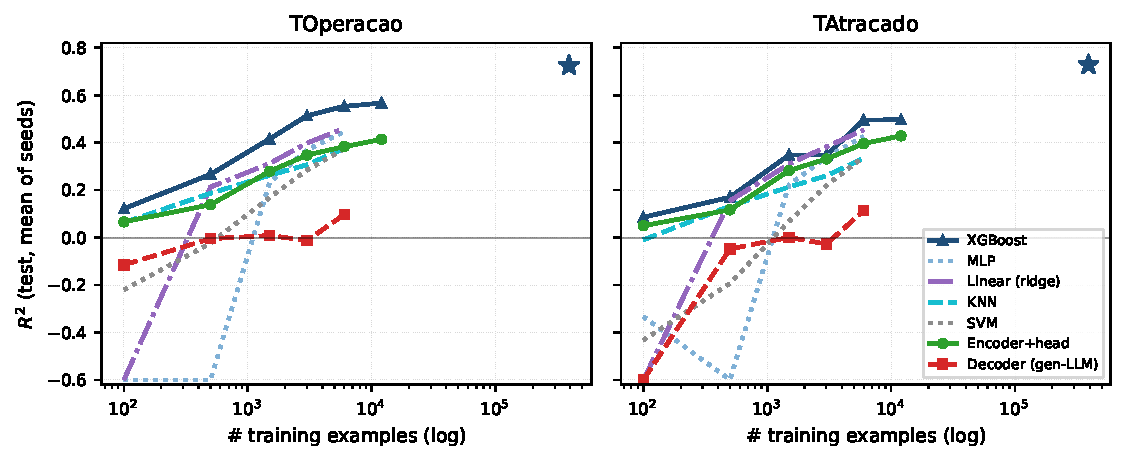
\includegraphics[width=0.99\columnwidth]{fig_allfamilies.pdf}
\caption{Data-matched data-efficiency ($R^2$ vs.\ number of training examples, log scale) for all seven model families trained on the \emph{same} $N$ random berthings ($100$--$6000$, 20 seeds); $\star$ is XGBoost's full-data point ($N{=}391{,}460$). XGBoost leads at every budget. The text encoder catches KNN/SVM by $N{=}6000$; linear and MLP overfit catastrophically at small $N$ in the $1606$-dim feature space (clipped at $-0.6$); the generative decoder stays near $0$ until a small rise at $6000$.}
\label{fig:curve}
\end{figure}

\subsection{ML versus text-based models}
Every ML model outperforms every text-based configuration on both targets. Table~\ref{tab:wilcoxon} compares XGBoost against the strongest configuration of each text family: all gaps are significant at $p<0.001$ with large pooled-$d$, and the RMSE deficit is $11$--$28$ hours. Even the weakest ML model (SVM, $R^2\approx0.48$) beats the best text-based model.

\begin{table}[t]
\centering
\caption{Paired comparison of XGBoost vs.\ each text-based configuration. $\Delta$RMSE $=$ mean(config)$-$mean(XGBoost) in hours (positive $=$ XGBoost better); $d$ is pooled Cohen's $d$; significance from paired Wilcoxon ($^{*}p{<}0.05$, $^{**}p{<}0.01$, $^{***}p{<}0.001$).}
\label{tab:wilcoxon}
\small
\begin{tabular}{@{}lcccc@{}}
\toprule
& \multicolumn{2}{c}{\texttt{TOperacao}} & \multicolumn{2}{c}{\texttt{TAtracado}} \\
\cmidrule(lr){2-3}\cmidrule(lr){4-5}
vs.\ XGBoost & $\Delta$RMSE & $d$ & $\Delta$RMSE & $d$ \\
\midrule
Encoder FT-12000    & +8.8 & -21.6$^{***}$ & +9.4 & -17.8$^{***}$ \\
Encoder FT-3000     & +10.3 & -15.2$^{***}$ & +11.9 & -14.8$^{***}$ \\
Encoder FT-100      & +16.1 & -19.0$^{***}$ & +18.2 & -17.2$^{***}$ \\
Gen-LLM FT-1500     & +17.1 & -9.0$^{***}$  & +19.2 & -10.9$^{***}$ \\
Gen-LLM FT-500      & +17.3 & -9.4$^{***}$  & +20.1 & -9.4$^{***}$ \\
Gen-LLM FT-100      & +19.2 & -8.3$^{***}$  & +28.3 & -2.7$^{***}$ \\
Qwen3-32B 0-shot    & +17.4 & -76.7$^{***}$ & +19.4 & -46.9$^{***}$ \\
Qwen3-32B 20-shot   & +17.2 & -8.5$^{***}$  & +20.5 & -6.2$^{***}$ \\
DeepSeek-V3 0-shot  & +17.3 & -66.2$^{***}$ & +21.1 & -116.1$^{***}$ \\
\bottomrule
\end{tabular}
\end{table}

\subsection{Prompting and fine-tuning data-efficiency}
\emph{In-context examples do not help.} For both frontier models, 5-shot and 20-shot are statistically indistinguishable from zero-shot (all $p>0.1$); 20-shot $\approx$ zero-shot and few-shot can destabilize DeepSeek-V3 (std up to $19$ h). \emph{Generative fine-tuning barely moves above $R^2\approx0$:} it rescues the small model from an unusable base ($R^2\approx-30$) but stays at $R^2\approx0$ through 3000 examples and only edges up to $\approx0.10$ at 6000 --- at or below the level of a 32B model prompted zero-shot. \emph{The encoder head is the exception:} its untrained base behaves as a mean predictor ($R^2\approx0$), and fine-tuning lifts $R^2$ monotonically and \emph{without saturating} across $100/500/1500/3000/6000/12000$ examples ($0.07\to0.14\to0.28\to0.35\to0.38\to0.41$ on \texttt{TOperacao}; $0.05\to0.12\to0.28\to0.33\to0.40\to0.43$ on \texttt{TAtracado}), beating the generative LLM at every budget (paired $p<0.01$; pooled $d$ from $-0.95$ to $-3.2$). Every doubling helps significantly --- even the $6000\to12000$ step ($p<0.05$, $d\approx0.9$) --- so the curve has not flattened. At 12000 examples ($R^2\approx0.41$--$0.43$) the encoder approaches the weakest ML models (SVM/linear, $R^2\approx0.48$--$0.52$), yet remains well below XGBoost's $0.73$, and the marginal gains are shrinking.

\noindent\emph{Data-matched comparison.} To separate representation from data budget, we train \emph{all seven families} on the same subsample sizes ($100$--$6000$ random berthings, 20 seeds, identical features for the ML models; Figure~\ref{fig:curve}, Table~\ref{tab:datamatched}). Four findings emerge. (i) XGBoost leads at \emph{every} budget --- already at $N{=}100$ ($R^2$ $0.12$ vs.\ the encoder's $0.07$) --- and is the most data-efficient: it reaches the encoder's $N{=}12000$ level ($R^2\approx0.42$) with only $\approx1500$ examples and trains $10$--$50\times$ faster (Table~\ref{tab:cost}). (ii) At small $N$ the high-dimensional ($1606$-feature) space breaks the linear and MLP models, whose unregularized/over-parameterized fits give large negative $R^2$ at $N\le500$; trees, KNN and the encoder stay robust. (iii) The text \emph{encoder} is competitive with standard ML at matched data --- by $N{=}6000$ it ($R^2\approx0.38$--$0.40$) matches KNN and SVM ($\approx0.34$--$0.38$), trailing only XGBoost, MLP and ridge. (iv) The generative \emph{decoder} stays at $R^2\approx0$ through $3000$ and only edges up at $6000$ ($\approx0.10$). The full ML model uses all $391{,}460$ berthings ($\star$); the largest data-matched budget here ($6000$) is $1.5\%$ of that, so the residual XGBoost-vs-encoder gap is both representational and one of budget. A log-linear fit of the encoder's $R^2$ against $\ln N$ extrapolates that matching XGBoost's full-data $R^2\approx0.73$ would take $\sim\!4\times10^5$ serialized examples (essentially the entire training set), while reaching the weakest ML tier ($R^2\approx0.5$) needs $\sim\!25{,}000$ ($\approx2\times$ our largest budget) --- and these are optimistic bounds, since the curve is already bending.

\begin{table}[t]
\centering
\caption{Data-matched test $R^2$ (mean over 20 seeds) by training-set size $N$, all families. Negative values ($<\!-1$) truncated. ML models share the engineered feature matrix; encoder/decoder read the serialized text.}
\label{tab:datamatched}
\small
\begin{tabular}{@{}lccccc@{}}
\toprule
& \multicolumn{5}{c}{$N$ (training examples)} \\
\cmidrule(lr){2-6}
\texttt{TOperacao} & 100 & 500 & 1500 & 3000 & 6000 \\
\midrule
XGBoost        & \textbf{0.122} & \textbf{0.267} & \textbf{0.416} & \textbf{0.514} & \textbf{0.553} \\
MLP            & --   & --   & 0.233 & 0.369 & 0.446 \\
Linear (ridge) & --   & 0.213 & 0.312 & 0.398 & 0.461 \\
KNN            & 0.064 & 0.187 & 0.262 & 0.307 & 0.375 \\
SVM            & -0.22 & -0.02 & 0.169 & 0.285 & 0.374 \\
Encoder        & 0.066 & 0.138 & 0.279 & 0.348 & 0.384 \\
Decoder (LLM)  & -0.12 & -0.01 & 0.009 & -0.01 & 0.097 \\
\midrule
\texttt{TAtracado} & 100 & 500 & 1500 & 3000 & 6000 \\
\midrule
XGBoost        & \textbf{0.086} & \textbf{0.170} & \textbf{0.348} & \textbf{0.348} & \textbf{0.495} \\
MLP            & -0.33 & --   & 0.223 & 0.338 & 0.426 \\
Linear (ridge) & -0.81 & 0.155 & 0.310 & 0.383 & 0.454 \\
KNN            & -0.01 & 0.133 & 0.213 & 0.261 & 0.334 \\
SVM            & -0.43 & -0.19 & 0.069 & 0.220 & 0.340 \\
Encoder        & 0.050 & 0.117 & 0.283 & 0.331 & 0.396 \\
Decoder (LLM)  & -0.64 & -0.05 & 0.001 & -0.03 & 0.113 \\
\bottomrule
\end{tabular}
\end{table}

\subsection{Computational cost}
Table~\ref{tab:cost} contrasts training and inference cost (local Apple M5 Pro for ML, encoder and generative LLM; Bedrock API for prompted LLMs; absolute values are not directly comparable across local vs.\ API, but orders of magnitude are). The encoder is the cheapest learned model (train $33$--$380$\,s, inference $<\!1$\,s for all 200 cases) and ML inference is sub-second; the generative LLM is by far the most expensive (train $\approx\!10$--$20$\,min at $3000$--$6000$ examples, $\approx\!20$\,s of autoregressive decoding for 200 cases) while being \emph{less} accurate, and prompted LLMs require an API round-trip per case that grows with the number of in-context examples. At the largest data-matched budget ($N{=}6000$) the contrast is stark: training takes $\approx\!4$\,s (XGBoost), $\approx\!290$\,s (encoder) and $\approx\!1170$\,s (generative LLM), while inference over the 200-case test set takes $\approx\!1$\,ms, $\approx\!0.9$\,s and $\approx\!20$\,s respectively.

\begin{table}[t]
\centering
\caption{Computational cost. Training is one-time (per seed for fine-tuning); inference is for the full 200-case test set unless noted. ML on CPU; encoder/generative LLM on M5 Pro (MPS); prompted LLMs via Bedrock.}
\label{tab:cost}
\small
\begin{tabular}{@{}lll@{}}
\toprule
Regime & Training & Inference (200 cases) \\
\midrule
XGBoost (ML)           & $182$ s ($+9$ s embed.) & $3$ ms \\
Encoder + head         & 33--380 s (100--12000) & $\approx 0.9$ s \\
Generative LLM (1.5B)  & 600--1170 s (3000--6000) & $\approx 20$ s \\
Prompted LLM (32B)     & none & $0.6$--$2.0$ s \emph{per case} \\
\bottomrule
\end{tabular}
\end{table}

\section{Discussion}
Three points stand out. First, \emph{representation, not model size, is decisive}: a 1.5B model fine-tuned on 1500 examples and a 32B model prompted with 20 examples both stall at $R^2\approx0$, while the small encoder reading the same text reaches $0.43$ (still rising at 12000 examples) and tuned trees reach $0.73$ --- the gains come from how cargo/route information is represented (dense embeddings, mass-weighted mixtures, target encoding) rather than from scale or prompting. Tellingly, XGBoost consumes the \emph{same} MiniLM embeddings \emph{frozen} (as features), whereas the encoder \emph{fine-tunes} that very backbone end-to-end with a regression head --- yet frozen-embeddings-plus-trees wins at every budget, indicating that the engineered tabular features and the tree's nonlinear interactions matter more than end-to-end adaptation of the text encoder. Second, \emph{a regression head matters and scales}: turning the task from text generation into supervised regression converts an LLM-family backbone from $R^2\le0$ into a model that improves monotonically with data, suggesting further gains with more examples --- but it remains text-only and does not see the engineered tabular features. Third, \emph{cost compounds the accuracy gap}: the most expensive learned model (generative LLM) is also the least accurate, whereas ML and the encoder are cheap to train and near-instant at inference.

\noindent\textbf{Limitations.} The comparison is deliberately asymmetric in representation: ML uses engineered features and embeddings, the text regimes read raw fields as text; this reflects how each family is used in practice. The test set has 200 fixed, leakage-free cases; seed sets differ across families and are paired by rank. We explored one small generative model and one encoder backbone under modest budgets; larger backbones, more examples, or hybrid text-plus-tabular models could narrow the gap and are left to future work.

\noindent\textbf{Practical implications and future work.} For heterogeneous operational-time prediction with a documented schema and abundant records, our results recommend tuned gradient boosting over semantic embeddings: it is both the most accurate and, at milliseconds per inference and minutes to train, by far the cheapest. Text-based models become attractive mainly in regimes this study does not target --- very low data, undocumented or shifting schemas, or zero-infrastructure settings --- where reading raw records as text sidesteps feature engineering. Promising directions include hybrid models that fuse the engineered tabular features with a fine-tuned text encoder, larger or instruction-tuned encoder backbones, and serializing the full training set to test whether the encoder's still-rising curve ultimately meets the tabular ceiling.

\section{Conclusion}
On a leakage-controlled seven-year ANTAQ benchmark for ship turnaround time, traditional ML with semantic embeddings decisively outperforms text-based models across prompting and fine-tuning: tuned XGBoost reaches $R^2\approx0.73$ while no prompted or generative-LLM configuration beats a mean predictor, and every gap is significant at $p<0.001$ with large effect size. An encoder with a regression head is the only text regime to extract real signal ($R^2$ up to $0.43$ and still rising at 12000 examples) and dominates the generative LLM at equal data and far lower cost, yet still trails all ML models. For heterogeneous operational-time regression of this kind, our evidence favors purpose-built ML with engineered semantic features over text-only models used as direct predictors.

\section{Code and Data}
All code, serialized prompts, per-seed predictions, metrics and the figures of this paper are released at \url{https://github.com/eduardocbpacheco/antaq-ml-vs-llm}~\cite{repo_code}. The underlying cleaned ANTAQ dataset (2018--2024) and the leakage-controlled processing pipeline are available on Zenodo (DOI \texttt{10.5281/zenodo.20549160})~\cite{zenodo_antaq}, and the corrected pipeline is detailed in~\cite{pacheco2026pitfalls}.

\begin{ack}
The authors thank ICMC--USP for computational support.
\end{ack}

\bibliographystyle{kdmile}
\bibliography{refs}

\begin{received}
\end{received}
\end{document}
